% !TeX spellcheck = en_US
\documentclass[]{article}

\usepackage[utf8]{inputenc}

\usepackage{natbib}
\usepackage{graphicx}

\usepackage[english]{babel}
\usepackage{amsmath}
\usepackage{amsfonts}
\usepackage{amssymb}

\usepackage[T1]{fontenc}
\usepackage{listingsutf8}
\lstset{literate={č}{{\v c}}1 {š}{{\v s}}1 {ž}{{\v z}}1}
\lstset{basicstyle=\ttfamily, language=matlab}


\title{Homework 1}
\author{Lovro Habjan}

\begin{document}

\maketitle


\section{Introduction}

For homework 1 we implemented iterative methods for tridiagonal matrices. We
wrote functions for \textit{Jacobi}, \textit{Gaus-Seidel} and \textit{SOR}
iterations.

\section{Methods}

Our goal is to solve the system $Ax = \mathbf{b}$ where $A \in \mathbb{R}^{n
\times n}$ is a tridiagonal matrix. For example
\begin{equation*}
	A = \begin{bmatrix}
		1 & 2 & 2 & 0 \\
		3 & 4 & 5 & 0 \\
		0 & 6 & 7 & 8 \\
		0 & 0 & 9 & 10
	\end{bmatrix}
\end{equation*}
which we can represent with matrix
\begin{equation*}
	M = \begin{bmatrix}
		0 & 1 & 2 \\
		3 & 4 & 5 \\
		6 & 7 & 8 \\
		9 & 10 & 0
	\end{bmatrix}
\end{equation*}

Because of this our iterative methods are easier to compute. If we observe the
equation for the Jacobian iteration
\begin{equation*}
	x_i^{(k+1)} = \frac{1}{a_{ii}} \left( b_i - \sum_{j = 1}^{i-1} a_{ij}
		x_j^{(k)} - \sum_{j = i + 1}^{n} a_{ij} x_j^{(k)} \right)
\end{equation*}
we observe that all elements $a_{i1}, a_{i2}, ..., a_{i i-2}, a_{i i + 2},
a_{i i + 3}, ..., a_{i n}$ equal 0 because $A$ is tridiagonal. This gives us
simpler equations for all three methods. Jacobian iteration looks like
\begin{equation*}
	x_i^{(k+1)} = \frac{1}{a_{ii}} \left( b_i - a_{i i-1} x_{i-1}^{(k)} -
		a_{i i+1} x_{i+1}^{(k)} \right),
\end{equation*}
Gauss-Seidel iteration as
\begin{equation*}
	x_i^{(k+1)} = \frac{1}{a_{ii}} \left( b_i - a_{i i-1} x_{i-1}^{(k+1)} -
		a_{i i+1} x_{i+1}^{(k)} \right)
\end{equation*}
and SOR iteration as
\begin{equation*}
	x_i^{(k+1)} = \frac{\omega}{a_{ii}} \left( b_i - a_{i i-1} x_{i-1}^{(k+1)} -
		a_{i i+1} x_{i+1}^{(k)} \right) + (1 - \omega) x_i^{(k)}
\end{equation*}


We use the maximum norm to stop the iteration when we achieve satisfactory
accuracy:
\begin{equation*}
	\Vert Ax^{(k)} - \mathbf{b} \Vert_{\infty} < acc
\end{equation*}


\section{Results}

All three methods are implemented in \textit{iter3.m} file. We count the number
of iterations for each method.

We tested our implementation with two examples. The test code is located in
\textit{test.m} file.

\subsection{Example 1 - small matrix}

We tested our implementation with the following system:
\begin{equation*}
		A = \begin{bmatrix}
	4 & 1 & 0 & 0 \\
	1 & 5 & -1 & 0 \\
	0 & -1 & 6 & 3 \\
	0 & 0 & 3	 & 7
	\end{bmatrix}
\end{equation*}
which takes the form:
\begin{equation*}
	M = \begin{bmatrix}
		0 & 4 & 1 \\
		1 & 5 & -1 \\
		-1 & 6 & 3 \\
		3 & 7 & 0
	\end{bmatrix}
\end{equation*}
Where $\mathbf{b}$ and solution $x$ is:
\begin{align*}
	\mathbf{b} = \begin{bmatrix}
		1 \\ 2 \\ 3 \\ 4
	\end{bmatrix}
	&
	x = \begin{bmatrix}
			0.1386 \\ 0.4457 \\ 0.3673 \\ 0.4140
	\end{bmatrix}
\end{align*}

Our initial guess is $x0 = \begin{bmatrix}
	0 & 0 & 0 & 0
\end{bmatrix}^T$. With $\omega = 1.5$ our implementation gives the following results:

\begin{lstlisting}
>> [x, j, g, s] = iter3(M, b, x0, 1e-13, 1.5)
x = [0.1386, 0.4457, 0.3673, 0.4140]
j = 46
g = 23
s = 46
\end{lstlisting}

We expirimentally determined the optimal value of $\omega$ by trying different
values from interval $(0, 2)$. Figure \ref{fig:1-omega} shows the results. We
see that the optimal value is $\omega = 1.1$.

\begin{figure}
	\centering
	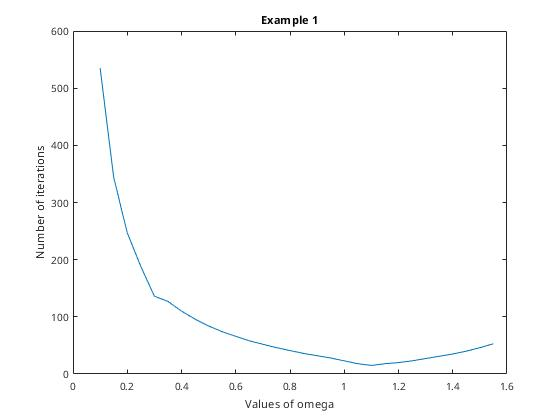
\includegraphics[width=\linewidth]{pics/test1-omega.jpg}
	\caption{Number of iterations for SOR method with different values of
		$\omega$ for example 1}
	\label{fig:1-omega}
\end{figure}


\subsection{Example 2 - big Laplace matrix}

For a bigger example we used a big Laplace matrix $A \in \mathbb{R}^{10^6 \times
10^6}$. Because of how we store the matrix it is only of size $10^6 \times 3$ of
form:

\begin{equation*}
	M = \begin{bmatrix}
		0 & 2 & -1 \\
		-1 & 2 & -1 \\
		-1 & 2 & -1 \\
		\vdots & \vdots & \vdots \\
		-1 & 2 & -1 \\
		-1 & 2 & 0
	\end{bmatrix}
\end{equation*}

right side is:
\begin{equation*}
	\mathbf{b} = \begin{bmatrix}
		1 & 0 & 0 & \cdots & 0 & 1
	\end{bmatrix}^T
\end{equation*}
and the solution is:
\begin{equation*}
	x = \begin{bmatrix}
		1 & 1 & \cdots & 1 & 1
	\end{bmatrix}^T
\end{equation*}

Our initial guess is:
\begin{equation*}
	x_0 = \begin{bmatrix}
		0 & 0 & \cdots & 0 & 0
	\end{bmatrix}^T
\end{equation*}

Our function returns the following:

\begin{lstlisting}
>> tic
>> [x, j, g, s] = iter3(M, b, x0, 1e-3, 1.7)
>> toc
Elapsed time is 35.683779 seconds.
j = 967
g = 254
s = 59
\end{lstlisting}

We experimentally determined that the value $\omega = 1.7$ is optimal, as is
shown in figure \ref{fig:2-omega}.

\begin{figure}
	\centering
	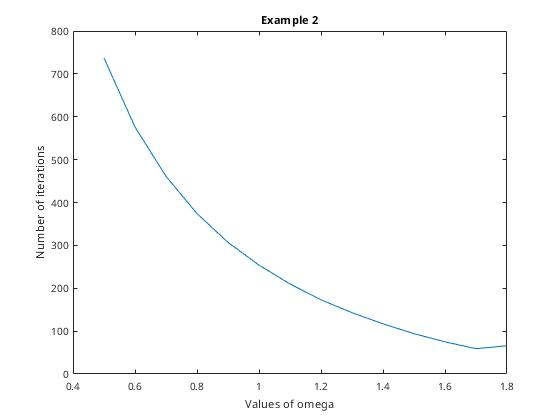
\includegraphics[width=\linewidth]{pics/test2-omega.jpg}
	\caption{Number of iterations for SOR method with different values of
		$\omega$ for example 2}
	\label{fig:2-omega}
\end{figure}

\end{document}
